\chapter{Introdução}\label{introducao}

Os túneis são grandes obras de engenharia que, além de causar grande admiração, atendem a diversas finalidades, sendo a mais conhecida aquela de transpor barreiras geológicas como, por exemplo, montanhas e canais marítimos, trazendo maior eficiência no transporte de recursos e pessoas. Também devido à crescente preocupação com o meio ambiente e com a preservação da superfície, essas estruturas têm sido cada vez mais empregadas em grandes cidades, melhorando assim a mobilidade urbana como, por exemplo, em metrôs e servindo de suporte para serviços públicos, tais como redes de água, esgoto, gás e eletricidade. São também empregados em hidroelétricas, laboratórios subterrâneos, instalações profundas para armazenamento de material radioativo e mineração.

Há, no entanto, um risco intrínseco associado a essas grandes obras, uma vez que o subsolo é em grande parte desconhecido e possui um comportamento complexo. Apesar de muitas dessas construções serem finalizadas com sucesso, ocorrem incidentes que levam a atrasos, custos excessivos e, em alguns casos, consequências mais significativas, tais como, danos em patrimônios de terceiros e perdas de vidas. Esses imprevistos estão relacionados a uma série de fatores que vão desde incertezas geológicas, cálculos inadequados, processo construtivo inapropriado e insuficiente monitoramento das deformações \textit{in loco}. Não obstante, uma parte destes acidentes está relacionada com a dificuldade em prever e modelar o comportamento mecânico dessas grandes obras.

Um dos comportamentos de difícil modelagem e ainda estudado é justamente a interação entre o comportamento instantâneo e o diferido dessas estruturas. Este comportamento pode ter um impacto significativo nas deformações e estabilidade da cavidade. A plastificação no entorno do maciço, o fechamento gradual da seção do túnel, a extrusão da face de escavação e a sobrecarga sobre o revestimento, podem se desenvolver durante o tempo construtivo, no curto prazo, ou ainda, meses e anos após a construção do túnel no médio e longo prazo. Esse comportamento pode causar deformações excessivas (\autoref{redução_base_turin}), danos ao revestimento (\autoref{ruptura_china}) e, em alguns casos, pela magnitude dos efeitos, acarretar o colapso da região no entorno do túnel.

\begin{figure}[H]
	\begin{center}
		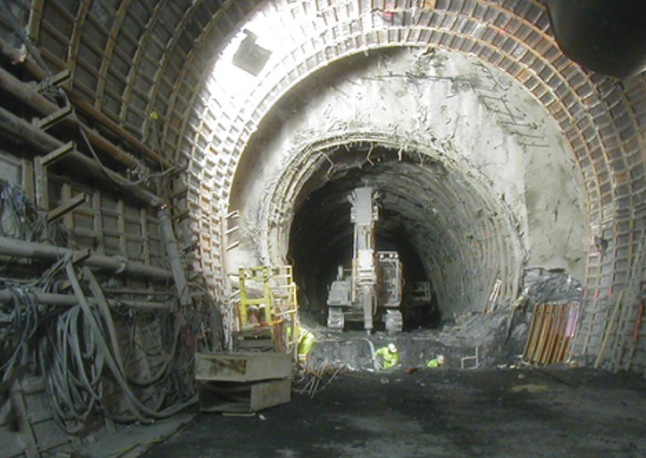
\includegraphics[width=12cm, height=8.33cm]{0101-redução da seção transversal do túnel de Base Lyon-Turin.png}
	\end{center}
	\caption{\label{redução_base_turin}Redução da seção transversal do Túnel de Base Lyon Turin na fronteira entre França e Itália (fonte: \citeonline[p. 41]{Barla2010})}
\end{figure}

\begin{figure}[H]
	\begin{center}
		\includegraphics[width=12cm, height=8.33cm]{0102-ruptura do suporte em uma mina de carvão na china.png}
	\end{center}
	\caption{\label{ruptura_china}Ruptura do suporte (perfil de aço) em uma mina de carvão na China (fonte: \citeonline[p. 192]{Manchao2015})}
\end{figure}
 
Além da estabilidade da cavidade, a escolha da tecnologia para a escavação é altamente influenciada pela magnitude dessa condição diferida no tempo. Por exemplo, em escavações com tuneladoras (TBM - \textit{Tunnel Boring Machines}), as pressões que se desenvolvem sobre a blindagem podem causar uma série de dificuldades como o aprisionamento da máquina (tal como visto em Ramoni e Anagnostou (\citeyear{Ramoni2010a,Ramoni2010b}). É sabido também que suportes flexíveis ou que apresentam um comportamento diferido no tempo (perfis metálicos deslizantes ou concreto projetado) são mais adequados do que suportes rígidos, uma vez que permitem um certo grau de acomodação dessas deformações diferidas.

Muitos estudos consideram leis constitutivas empírico-experimentais, viscoelásticas ou ainda viscoplásticas em suas análises diferidas no tempo, contudo, todos esses modelos partem de um comportamento instantâneo elástico o que pode não corresponder com a realidade, uma vez que o maciço pode possuir um comportamento instantâneo elastoplástico induzido pelo processo construtivo.

Em vista da importância do tema para a comunidade geotécnica de túneis, a presente tese desenvolve uma relação constitutiva para lidar com o comportamento diferido no tempo, considerando um modelo viscoplástico, conjuntamente com o comportamento instantâneo dado por um modelo elastoplástico. Portanto, um modelo constitutivo acoplado.

Além dessa introdução, esse trabalho está dividido em mais 7 capítulos.

O \textbf{capítulo 2} tem a finalidade de esclarecer o mais objetivamente possível o que se pretende desenvolver nessa tese, explicitando o tema, os objetivos a alcançar, as delimitações  adotadas e o delineamento de como se deu o trabalho.

O \textbf{capítulo 3} foi introduzido com o intuito de apresentar brevemente alguns aspectos do estado da arte de túneis. Portanto, esse capítulo resume brevemente os métodos de escavação, os elementos e técnicas de pré-suporte, os revestimentos e principais aspectos considerados em estudos numéricos recentes. Portanto, esse capítulo é opcional aos leitores mais experientes e pode ser ignorado sem prejuízo ao entendimento do trabalho restante.

O \textbf{capítulo 4} tem por finalidade instruir o leitor no comportamento mecânico de túneis e seus conceitos fundamentais. Esse capítulo está dividido de acordo com os principais fatores que influenciam o campo de tensões e deformações no entorno dessas estruturas, tais como, o processo de escavação, o comportamento reológico do maciço, a forma da seção, a profundidade do túnel, a proximidade da superfície e a interação com o revestimento. Nesse capítulo é dada uma maior ênfase na reologia do maciço, caracterizando o comportamento instantâneo e diferido, que são justamente os comportamentos almejados no modelo proposto dessa tese. Ao final, também são apresentados alguns estudos que consideraram leis elastoplástica-viscoplástica no comportamento do maciço.

O \textbf{capítulo 5} descreve o modelo teórico implementado esclarecendo as principais hipóteses e explicando cada uma das leis constitutivas adotadas (elástica, elastoplástica e viscoplástica) de forma genérica e separada. No final desse capítulo é descrito então o modelo constitutivo acoplado elastoplástico-viscoplástico desenvolvido nessa tese.

O \textbf{capítulo 6} se refere à solução numérica do modelo teórico implementado. Portanto, descreve a discretização espacial em elementos finitos, incluindo os tipos de elementos que são utilizados, o método de solução do sistema não linear e o algoritmo de integração das leis constitutivas. Esse último é um dos principais focos do trabalho, uma vez que nele é feita a junção entre o modelo elastoplástico (instantâneo) e o viscoplástico (diferido). Também nesse capítulo são apresentadas as malhas propostas para as análises de túneis profundos (estado plano de deformação, tridimensional e axissimétrico) bem como as condições de contorno utilizadas e a descrição do processo de escavação e colocação do revestimento pelo método da ativação e desativação de elementos. No final é apresentado os principais parâmetros do modelo constitutivo implementado.

O \textbf{capítulo 7} mostra algumas validações e verificações do algoritmo implementado com soluções analíticas para túneis profundos e soluções numéricas obtidas pelo \textit{software} de elementos finitos GEOMEC91\footnote{O GEOMEC91 é um \textit{software} de elementos finitos para análises de túneis em axissimetria desenvolvido por \citeonline{Bernaud1991}.} desenvolvido por \citeonline{Bernaud1991}. A verificação do modelo acoplado é feita através de uma solução analítica e numérica desenvolvida por \citeonline{Piepi1995}. Essa validação é apenas parcial, uma vez que essa solução é menos geral que o modelo consitutivo implementado, pois considera o comportamento elastoplástico-viscoplástico perfeito associado obedecendo apenas ao critério de Tresca. Contudo, é importante para demonstrar que o algoritmo acoplado está funcionando. Também nesse capítulo são feitas algumas análises paramétricas, incluindo, túneis com seção transversal elíptica.

Por fim, o \textbf{capítulo 8} faz o fechamento da tese apresentando algumas conclusões e sugestões de trabalhos futuros.


 
